

\chapter{Introduction}
\labch{introduction}

\begin{margintable}[*8.5]
  \caption{Cost to fix bugs at different development stages \cite{White2017}.}
  \labtab{effort-to-fix}
  \centering
  \resizebox{\textwidth}{!}{
  \begin{tabular}{c c}
    \toprule
    \textsc{Bug Found at Stage} & \textsc{Cost to Fix} \\
    \midrule
    Requirements & 1x (definition) \\
    Architecture & 3x \\
    Design & 5-10x \\
    System Test & 10x \\
    Production & 10-100x \\
    \bottomrule
  \end{tabular}
  }
\end{margintable}

Recent advances and evolution in software development have led to increasingly complex software systems.
The reliability of these systems is based on their correctness.
Any failure or vulnerability in software poses significant risks, potentially threatening human safety or causing financial losses.
As software grows in complexity, the likelihood of bugs also increases.
The effort and cost to fix these bugs escalate with late detection, as illustrated in \reftab{effort-to-fix} \sidecite[*10.4]{White2017}, which shows the relative costs of fixing bugs at different development stages.
Today, software rules safety-critical systems such as nuclear power plants \sidecite[*10.3]{Krasner2021},
car engines \sidecite[*12.3]{Finch2009},
airplane control systems
\sidecite[*14.9]{Briere1993},
and medical devices \sidecite[*17.7]{Leveson1993}.
For systems where safety is critical, addressing bugs before deployment is mandatory.

Machine learning software is increasingly impacting society by assisting or even automating decision-making in fields such as social welfare \sidecite[*16.3]{Larson2016}, criminal justice \sidecite[*17.4]{Buolamwini2018}, and healthcare \sidecite[*21]{Obermeyer2019}.
However, recent cases have shown that such software can reproduce or even reinforce biases present in the training data \cite{Buolamwini2018,Kay2015,Larson2016,Obermeyer2019}\phantomcite[*22]{Kay2015}.
In April 2021, the European Commission proposed the Artificial Intelligence Act~\sidecite[*23.9]{Commission2021}, a first legal framework on machine learning software, imposing strict requirements to minimize the risk of discriminatory outcomes.


Moreover, recent advancements in artificial intelligence have led to the rise of large language models (LLMs) capable of generating software from natural language specifications.
Agents like OpenAI's ChatGPT and Google's Gemini are gaining widespread use.
Specifically designed for coding, GitHub Copilot assists programmers within IDEs and has over a million subscribers.
Despite their benefits, AI-generated code can introduce as many bugs as human-written code, making it crucial to use techniques that detect software errors or certify intended behaviors.

\section{Software Quality}

Software quality measures how well software meets its requirements.
The most common method to ensure software quality is \emph{testing}.
The correct behavior of software is tested empirically for a finite number of inputs against a set of assertions specifying the functional requirements of the code.
However, testing has inherent limitations.
It can only verify a program against functional requirements, which may be poorly defined and ambiguous, leading to inadequate testing.
Exhaustive testing is impractical, and constraints on time and budget can further impact the process.
Mostly, testing cannot guarantee the absence of bugs\sidenote[][*3]{``Program testing can be quite effective for showing the presence of bugs, but is hopelessly inadequate for showing their absence.'' -- \textcite{Dijkstra1976}} \sidecite[*6.5]{Dijkstra1976}.
While in some cases it is acceptable to deploy software with bugs (relying on patches to fix them, \reftab{effort-to-fix}), in safety-critical systems, it is necessary to ensure that the software is free of bugs before deployment to avoid catastrophic consequences.

In contrast to testing, \emph{formal methods} provide rigorous mathematical guarantees about software correctness.
Thanks to their mathematical foundation, formal methods guarantee 100\% accuracy in verifying software properties.
The idea of formally verifying software dates back to the late 1960s with program proofs and invariants from \sidetextcite{Floyd1967} and \sidetextcite{Hoare1969}.
Even earlier, formal methods can be traced to the work of \sidetextcite{Church1936} and \sidetextcite{Turing1937} on the foundations of computation.
According to software engineering practices, formal methods can be introduced early in the development lifecycle, enabling the verification of software properties at the design stage.

\begin{center}\em
  Why should formal methods replace other well-known, widely accepted, and user-friendly techniques such as testing?
\end{center}

To answer this question, consider the following examples where testing failed:

\begin{itemize}
\item The Ariane 5 rocket failure in 1996, caused by an integer overflow bug, resulted in a loss of \$370 million\sidenote{\url{https://esamultimedia.esa.int/docs/esa-x-1819eng.pdf}}.
\item The crash of Air France Flight 447 in June 2009, killing hundreds of passengers, was due to a probe sensor failure that was not detected during testing, as test engineers assumed such a failure was impossible \sidecite{Charette2009}.
\item The Therac-25 radiation therapy machine malfunctioned due to software bugs, resulting in patient deaths and serious injuries \sidecite{Leveson1993}.
\item The Toyota unintended acceleration case, where a stack overflow resulted in the death of 89 people and a lawsuit of \$1.2 billion\sidenote{\url{https://www.embeddedrelated.com/showarticle/1574.php}}.
\item A round-off error in the Patriot missile system caused the death of 28 people during the Gulf War\sidenote{\url{https://www.ima.umn.edu/~arnold/disasters/patriot.html}}.
\end{itemize}

These cases could have been avoided with formal methods.

Unlike testing, formal methods enable exhaustive search and detection of bugs that testing may miss.
System requirements are translated into formal specifications, which are mathematically verified to ensure the system's behavior aligns with real-world scenarios.
However, Rice's undecidability theorem \sidecite{Rice1953} states that all non-trivial properties\sidenote{A property is non-trivial if it is not true for all programs or false for all programs.} are undecidable, meaning there is no terminating algorithm that can decide whether a program satisfies a non-trivial property.
Consequently, formal methods either sacrifice \emph{completeness}, \emph{soundness}, or \emph{automation}.
Current formal methods can be classified into three categories \sidecite{Cousot2010} (\reffig{formal-methods-trade-offs}): \emph{theorem provers}, \emph{model checking}, and \emph{static analysis}.

\begin{marginfigure}
  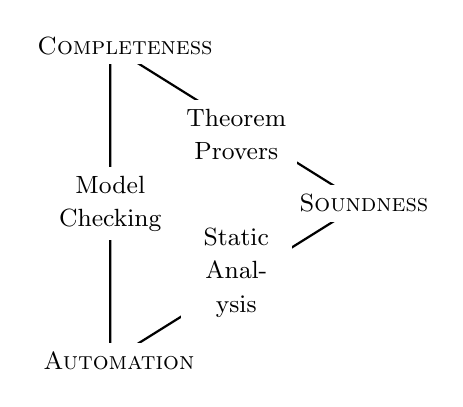
\begin{tikzpicture}[scale=0.8]
    % Draw the triangle
    \draw[thick] (0,0) -- (4,2.5) -- (0,5) -- cycle;

    % Place the vertices with blue squared borders
    \node[draw, fill=white, text width=1.7cm, align=center, draw=white] at (0,0) {\small \textsc{Automation}};
    \node[draw, fill=white, text width=1.6cm, align=center, draw=white] at (4,2.5) {\small \textsc{Soundness}};
    \node[draw, fill=white, text width=1.85cm, align=center, draw=white] at (0,5) {\small \textsc{Completeness}};

    % Place the edges' labels inside the edges
    \node[fill=white, text width=1.18cm, align=center] at (2,1.4) {\small Static Analysis};
    \node[fill=white, text width=1.5cm, align=center] at (0,2.5) {\small Model Checking};
    \node[fill=white, text width=1.3cm, align=center] at (2,3.6) {\small Theorem Provers};
\end{tikzpicture}
  \caption{Trade-offs in formal methods.}
  \labfig{formal-methods-trade-offs}
\end{marginfigure}

Theorem provers \sidecite{Nawaz2019} produce proofs of correctness using interactive tools, also called proof assistants, such as Coq \sidecite{Bertot2004} and HOL Light \sidecite{Harrison2009}, or automatic ones \sidecite{Sutcliffe2001}.
User interaction is ultimately required to guide the proof search in both the interactive and automatic cases.
Theorem provers are complete and sound but not fully automated.

Formal methods based on model checking automatically explore the state space of a program's model to verify whether undesirable states are reachable.
\sidetextcite{Clarke2004} applied model checking to prove the correctness of ANSI-C programs.
However, model checking methods are limited by the state explosion problem: the number of feasible execution paths grows exponentially with the model's size, trading soundness for completeness and automation.

Static analysis analyzes the program source code to some level of abstraction without user interaction.
This abstraction is sound but incomplete, meaning the analysis may report \emph{false alarms}, \ie, warnings that a correct program may be incorrect.
However, whenever the static analysis certifies the absence of a bug, the program is indeed bug-free.
The most common static analysis techniques are based on \emph{abstract interpretation}.

Abstract Interpretation \sidecite{Cousot1977} is a general theory for approximating program semantics, developed by Patrick and Radhia Cousot in the late 1970s, see \sidecite{Cousot2024} for an historical view on abstract interpretation.
Their framework is based on the observation that not all computational details are necessary to reason about program properties.
Instead, the program's semantics can be approximated by a simpler, more abstract model that facilitates automatic reasoning.

Over the past decade, abstract interpretation-based static analyses have been successfully applied to real-world software development.
The \emph{Astrée} static analyzer \sidecite{Blanchet2003} is routinely used to ensure the absence of runtime errors in embedded synchronous C programs for the Airbus A340 and A380.

We provide a formal introduction to abstract interpretation in \refch{abstract-interpretation}, recalling the main results used in this thesis, illustrated on a small idealized programming language at the end of the chapter.

\section{Input Data Usage}

Programming errors in software systems do not always result in crashes or runtime errors.
Sometimes, faulty programs produce plausible yet erroneous outcomes or unsafe behaviors.
Such bugs are hard to spot since they provide no clear indication that something went wrong.
A potential source of such errors is the misuse of input data, \ie, when an input variable has an unexpected impact on the program computation compared to the developers' expectations.

A notable example is the Reinhart and Rogoff article “Growth in a Time of Debt” \sidecite{Reinhart2010}, which claimed that economic growth is negatively correlated with public debt.
This article was heavily cited to justify austerity measures worldwide in the following years.
However, in 2013, \sidetextcite{Herndon2014} discovered that the authors had made a mistake in their Excel spreadsheet, leading to the erroneous conclusion.
One of the errors was the incorrect usage of the input value relative to Norway's economic growth in 1964, with an excessive weight in the average growth rate computation.

In data science applications, where software involves long pipelines that filter, merge, and manipulate data, programming errors causing input variables to have more or less influence than expected are likely.
Hence, it is essential to employ techniques that enhance confidence in the usage of input variables for data-driven applications.

\refch{input-data-usage} introduces the input data usage property, a formal property that captures the \emph{qualitative} usage of input data in a program.

\section{Quantitative Properties}

Typically, program properties are qualitative; a program either satisfies a property or not.
This constraint is not always sufficient to capture the complexity of real-world requirements \sidecite{Smith2007}.
For instance, one fundamental security issue is protecting sensitive information confidentiality.
Secure information flow analysis questions whether a program could leak information about its secrets.
Noninterference, certifying that a program reveals no information about its secrets, is a classic approach.
However, noninterference is too strict for many practical applications.
For example, in a digital election protocol, individual votes should be anonymous, but the final result needs to be revealed.
A password checker should not reveal the password but should indicate whether the password is correct.
These cases represent deliberate violations of noninterference necessary for the program to fulfill its purpose.

To address this limitation, quantitative properties are considered \sidecite{Smith2009}.
The key idea is to accept that a program may violate a property and compare such violation against a threshold.
Programs are classified as \emph{safe} or \emph{unsafe} based on the degree of violation, inducing a classification among programs based on how much safety they provide.

In the Reinhart and Rogoff case, the value of Norway's economic growth was indeed used in the average computation, but its impact was much higher than it should have been.
The error was not whether the value was used but rather how much it was used.
A quantitative analysis would have revealed that the impact of Norway's economic growth was too high, allowing the authors to correct the wrong conclusion.

\refch{quantitative-input-data-usage} introduces the formal framework, based on abstract interpretation, to reason about quantitative properties of programs' input data usage.

\section{Outline and Contributions}

In this thesis, we study formal reasoning techniques to detect input data misuse.
We propose semantics-based static analysis techniques to quantify the impact of input variables on program computation.
In \arefpart{background},
\refch{abstract-interpretation} provides the mathematical background used in the rest of the thesis and introduces the abstract interpretation framework.
In \arefpart{conclusion}, \refch{related-work} discusses related work, and \refch{conclusion} concludes the thesis with a summary and future work.
The rest of this section outlines the thesis's main body.

\subsection{Input Data Usage}

In \arefpart{background}, \refch{input-data-usage} defines the input data usage property as proposed by \sidetextcite{Urban2018}.
We extend the property to capture abstractions of output values, similarly to the generalization of non-interference \sidecite{Giacobazzi2018}, discussing relations between the two properties.
We provide a hierarchy of semantics that precisely captures the input data usage property, abstracting unnecessary details.
Finally, we report an abstract semantics that captures syntactic dependencies between variables from \textcite{Urban2018}, used to approximate the input data usage property soundly.

\subsection{Quantitative Verification of Extensional Properties}[Extensional Properties]

In \arefpart{extensional}, we focus on the quantitative verification of extensional properties, \ie, properties that depend on the input-output behavior of a program.
This part is divided into three chapters: the first one presenting the novel quantitative framework, the second applying the framework to neural networks, and the third showing the experimental evaluation of this part.

\paragraph{Quantitative Input Data Usage}
In \refch{quantitative-input-data-usage}, we present a novel quantitative input usage framework to discriminate between input variables with different impacts on a program's outcome.
This framework can identify variables with disproportionate impact, certifying intended behavior or revealing potential flaws by matching developers' expectations with actual results.
We characterize the impact of an input variable with a notion of dependency between variables and program outcomes.
Our framework is parametric in the impact definition of choice.
%
We introduce a backward static analysis based on abstract interpretation, parametric in the impact definition, which infers a sound over-approximation of the impact of input variables.
The analysis computes the input states leading to output buckets, applying a computable implementation of the impact on the backward reachability analysis result.
This approach allows end-users to choose the impact that fits their needs, ensuring a targeted and customizable analysis.
\marginnote[*-13]{\refch{quantitative-input-data-usage} is based on work published at NASA Formal Methods
Symposium (NFM) 2024 \cite{Mazzucato2024b}.}
\marginnote[*-10.5]{\formatmargincitation{Mazzucato2024b}}


\paragraph{Quantitative Verification for Neural Networks}
In \refch{quantitative-fairness}, we extend the quantitative input data usage property to neural networks.
We propose two impact notions for neural networks, addressing the ragged input space and measuring input features' fairness.
We refine the backward analysis to exploit parallel computations for better performance, employing a combination of forward and backward analyses.
The forward pass reduces the backward analysis's combinatorial explosion, partitioning the input space into subregions for easier parallel analysis.
\marginnote[*-7]{\refch{quantitative-fairness} is based on work published at the 28th Static Analysis Symposium (SAS) 2021 \cite{Mazzucato2021}.}
\marginnote[*-4.5]{\formatmargincitation{Mazzucato2021}}


\paragraph{Experimental Evaluation of Extensional Properties}
\refch{extensional-eval} demonstrates the quantitative framework's potential applications by evaluating our static analysis tool, \impatto, against six use cases, and presents our approach's evaluation on neural networks.

\subsection{Quantitative Verification of Intensional Properties}[Intensional Properties]

\marginnote{\arefpart{intensional} is based on work published at the 31st Static Analysis Symposium (SAS) 2024 \cite{Mazzucato2024a}.}
\marginnote{\formatmargincitation{Mazzucato2024a}}

\arefpart{intensional} focuses on the quantitative verification of intensional properties, \ie, properties that depend on the program's internal behavior, \eg, the number of iterations of a loop.
This part is divided into two chapters: the first one presenting the novel quantitative timing analysis, and the second showing the experimental evaluation.

In \refch{quantitative-static-timing-analysis}, we consider the number of program iterations as the program outcome, capturing the impact of input variables on the global number of iterations.
This variation is crucial, as programming errors affecting iterations can degrade performance or introduce security vulnerabilities without functional errors.
For instance, unexpected input impacts on runtime could reveal sensitive information \sidecite{Wong2005}, posing security threats.
Even cryptographic programs are vulnerable to timing attacks, depending on implementation choices.
\sidetextcite{Kocher1996} demonstrated that public key cryptographic algorithms, like RSA, are susceptible to timing attacks, potentially leaking secret keys.

Knowing the timing behavior of a program can certify intended behavior or reveal latent flaws by matching developers' expectations with actual program behavior.
For performance optimization, identifying input variables that significantly affect loop iterations helps developers focus on critical code segments \sidecite{Omar2017}.
Consequently, understanding the impact of input variables on runtime is paramount.
In this study, we focus on quantifying input variables' impact on loop iterations as an indicator of runtime behavior.

We leverage global loop bound analysis to derive an over-approximation of the global loop bound, encoding the quantification of input variables' impact as a linear programming problem.
Our approach blends syntactic and semantic information: generating invariants as linear constraints for accuracy and combining global loop bound analysis with syntactic dependency analysis \sidecite{Urban2018} for scalability.

In \refch{intensional-eval}, we present \timesec, a tool implementing our quantitative timing analysis.
We demonstrate its effectiveness in a real-world cryptographic library, certifying its immunity to timing side-channel attacks by showing no impact of input variables on loop iterations.
Additionally, we evaluate \timesec{} against programs from \svcomp.

\subsection{Contributions}

The main contributions of this thesis are as follows:
\begin{itemize}
  \item In \refch{input-data-usage}, we extend the original definition of the input data usage property to capture abstractions of output values.
  Such extension blends generalized non-interference with input data usage, providing a definition that works also for non-deterministic programs.
  \item In \arefpart{extensional}:
    \begin{itemize}
      \item In \refch{quantitative-input-data-usage}, we develop a theoretical framework by abstract interpretation to quantify the impact of input variables by considering three novel impact notions.
      \item In \refch{quantitative-input-data-usage}, we present our static analysis and a possible abstract implementation of the impact instances; to showcase our approach we implement a tool called \impatto\sidenote{\impattourl}.
      \item In \refch{quantitative-fairness}, we present two impact notions for neural networks.
      \item In \refch{quantitative-fairness}, we propose an improved backward analysis that exploits parallel computations and achieves better precision by combining abstract domains; this extension is part of the \libra\sidenote{\libraurl} tool.
    \end{itemize}
  \item In \arefpart{intensional}:
    \begin{itemize}
      \item we propose a static analysis, employing a linear constraint abstract domain, global loop bound analysis, and linear programming encoding to quantify the impact of input variables on loop iterations, and
      \item we present \timesec\sidenote{\timesecurl}, a tool implementing our quantitative timing analysis, and evaluate it against the \bignum{} cryptographic library\sidenote{\bignumurl} and programs from \svcomp \sidenote{\svcompurl}.
    \end{itemize}
\end{itemize}
